\documentclass[11pt,a4paper]{article}

\usepackage[margin=1.85cm,top=2.1cm,bottom=2.2cm]{geometry}
\usepackage[T1]{fontenc}
\usepackage[utf8]{inputenc}
\usepackage{lmodern}
\usepackage{microtype}
\usepackage{graphicx}
\usepackage{xcolor}
\usepackage{booktabs}
\usepackage{array}
\usepackage{tabularx}
\usepackage{longtable}
\usepackage{enumitem}
\usepackage{fancyhdr}
\usepackage{titlesec}
\usepackage{hyperref}
\usepackage{listings}
\usepackage[most]{tcolorbox}

\definecolor{navy}{HTML}{0F172A}
\definecolor{slate}{HTML}{475569}
\definecolor{muted}{HTML}{64748B}
\definecolor{line}{HTML}{CBD5E1}
\definecolor{soft}{HTML}{F8FAFC}
\definecolor{blue}{HTML}{2563EB}
\definecolor{teal}{HTML}{0D9488}
\definecolor{amber}{HTML}{D97706}
\definecolor{codebg}{HTML}{F1F5F9}

\hypersetup{
    colorlinks=true,
    linkcolor=blue,
    urlcolor=teal,
    citecolor=blue,
    pdftitle={MLOps Exam Project Report},
    pdfauthor={Ayoub Moutik}
}

\pagestyle{fancy}
\fancyhf{}
\lhead{\textcolor{slate}{MLOps Exam Project}}
\rhead{\textcolor{slate}{MLOps Workflow Report}}
\cfoot{\textcolor{slate}{\thepage}}
\renewcommand{\headrulewidth}{0.4pt}
\renewcommand{\headrule}{\hbox to\headwidth{\color{line}\leaders\hrule height \headrulewidth\hfill}}

\titleformat{\section}
  {\Large\bfseries\color{navy}}
  {\thesection}{0.8em}{}
  [\vspace{-0.4em}{\color{line}\titlerule}]

\titleformat{\subsection}
  {\large\bfseries\color{navy}}
  {\thesubsection}{0.7em}{}

\titleformat{\subsubsection}
  {\normalsize\bfseries\color{navy}}
  {\thesubsubsection}{0.6em}{}

\setlist[itemize]{leftmargin=1.4em,itemsep=0.25em,topsep=0.25em}
\setlist[enumerate]{leftmargin=1.5em,itemsep=0.25em,topsep=0.25em}
\renewcommand{\arraystretch}{1.25}

\lstdefinestyle{projectcode}{
    backgroundcolor=\color{codebg},
    basicstyle=\ttfamily\small,
    keywordstyle=\color{blue}\bfseries,
    commentstyle=\color{muted},
    stringstyle=\color{teal},
    breaklines=true,
    frame=single,
    rulecolor=\color{line},
    frameround=tttt,
    columns=fullflexible,
    showstringspaces=false,
    tabsize=2
}

\newtcolorbox{infobox}[1]{
    enhanced,
    colback=soft,
    colframe=line,
    coltitle=navy,
    fonttitle=\bfseries,
    title=#1,
    arc=2mm,
    boxrule=0.6pt,
    left=3mm,
    right=3mm,
    top=2mm,
    bottom=2mm
}

\begin{document}

\begin{titlepage}
    \pagecolor{soft}
    \begin{center}
        \vspace*{1.4cm}
        {\Huge\bfseries\color{navy} MLOps Exam Project Report}\\[0.35cm]
        {\Large\color{slate} From Notebook Experimentation To Reproducible ML Workflows}\\[1.2cm]

        \begin{tcolorbox}[
            enhanced,
            width=0.86\textwidth,
            colback=white,
            colframe=line,
            arc=3mm,
            boxrule=0.8pt,
            left=8mm,
            right=8mm,
            top=7mm,
            bottom=7mm
        ]
            \centering
            {\Large\bfseries\color{blue} End-To-End MLOps Workflow}\\[0.25cm]
            \textcolor{navy}{A structured implementation report for a machine learning text classification system.}\\[0.35cm]
            \textbf{Code Organization} \quad
            \textbf{Logging} \quad
            \textbf{Reproducibility} \quad
            \textbf{Automation}
        \end{tcolorbox}

        \vfill
        \begin{tabular}{rl}
            \textbf{Student:} & Ayoub Moutik \\
            \textbf{Course:} & DevOps / MLOps \\
            \textbf{Project:} & MLOpsFull and Monitoring-ML \\
            \textbf{Date:} & May 13, 2026 \\
        \end{tabular}
        \vspace*{1cm}
    \end{center}
    \nopagecolor
\end{titlepage}

\tableofcontents
\newpage

\section*{Abstract}
\addcontentsline{toc}{section}{Abstract}

This report presents the design and implementation of an MLOps workflow for a machine learning text classification project. The system is organized around a modular Python codebase that supports data processing, model training, evaluation, prediction, and serving. The workflow emphasizes maintainability, traceability, and reproducibility, which are essential requirements for reliable machine learning systems.

The report begins by describing the project architecture and the transition from notebook-based experimentation to script-based engineering. It then presents the logging strategy used to capture execution details and operational events. Finally, it analyzes the reproducibility mechanisms provided by Git, dependency management, MLflow tracking, model checkpointing, dataset organization, and deterministic utilities.

\section{Project Context And Objective}

\subsection{Context}

The project material is composed of five course PDFs and two repositories:

\begin{itemize}
    \item \texttt{MLOpsFull}: the main machine learning application.
    \item \texttt{Monitoring-ML}: a monitoring notebook and README covering model performance, drift detection, and online monitoring.
\end{itemize}

The main application is a text classification system inspired by the Made With ML project. It classifies machine learning project descriptions into tags such as computer vision, natural language processing, graph learning, MLOps, reinforcement learning, and other categories.

\subsection{Objective}

The objective is to demonstrate an end-to-end MLOps workflow. The project includes the foundational engineering practices required before automation and monitoring can be introduced reliably:

\begin{enumerate}
    \item moving from notebooks to scripts;
    \item logging for ML systems;
    \item reproducibility through versioned code, data, models, and dependencies.
\end{enumerate}

\begin{figure}[h]
    \centering
    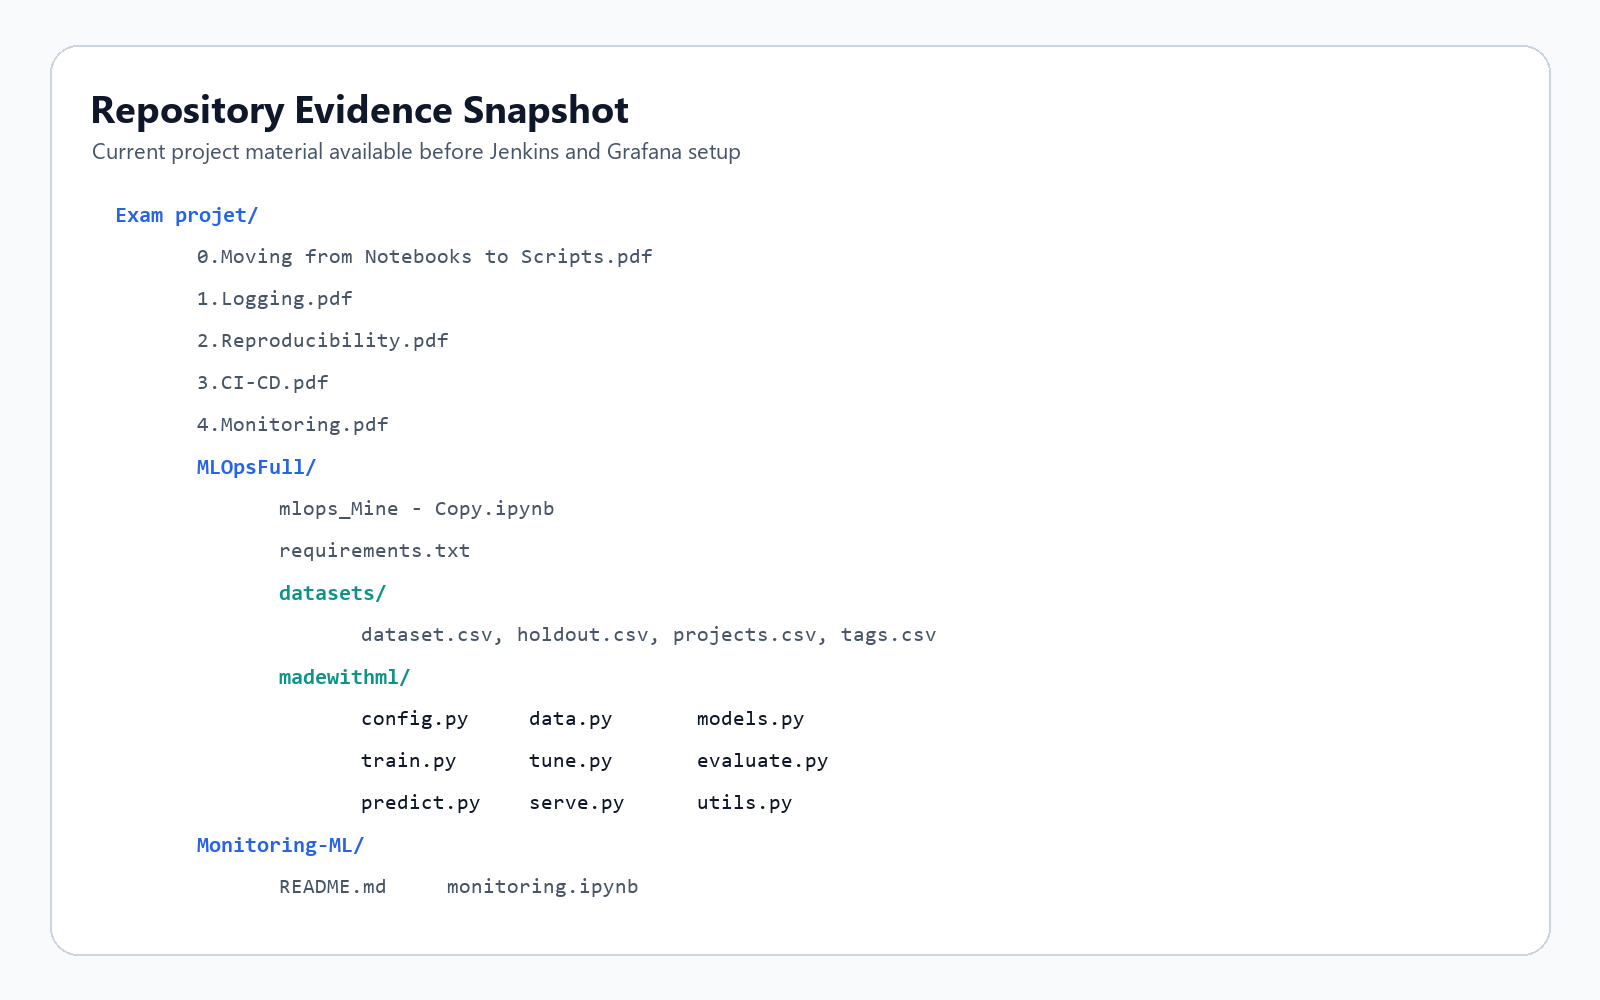
\includegraphics[width=0.92\textwidth]{figures/repository_snapshot.png}
    \caption{Current project material available in the workspace.}
    \label{fig:repo-snapshot}
\end{figure}

\section{Part 1: Moving From Notebooks To Scripts}

\subsection{Purpose}

Notebooks are excellent for exploration because they allow interactive execution, visual inspection, and fast experimentation. However, they are not ideal as the final structure of a production ML project. A notebook can hide execution order, retain variables in memory, and make testing or automation difficult.

Scripts provide a cleaner engineering structure. They make workloads easier to test, execute from a terminal, reuse in CI/CD, and deploy as services. This is the first major step from data science experimentation toward MLOps.

\begin{figure}[h]
    \centering
    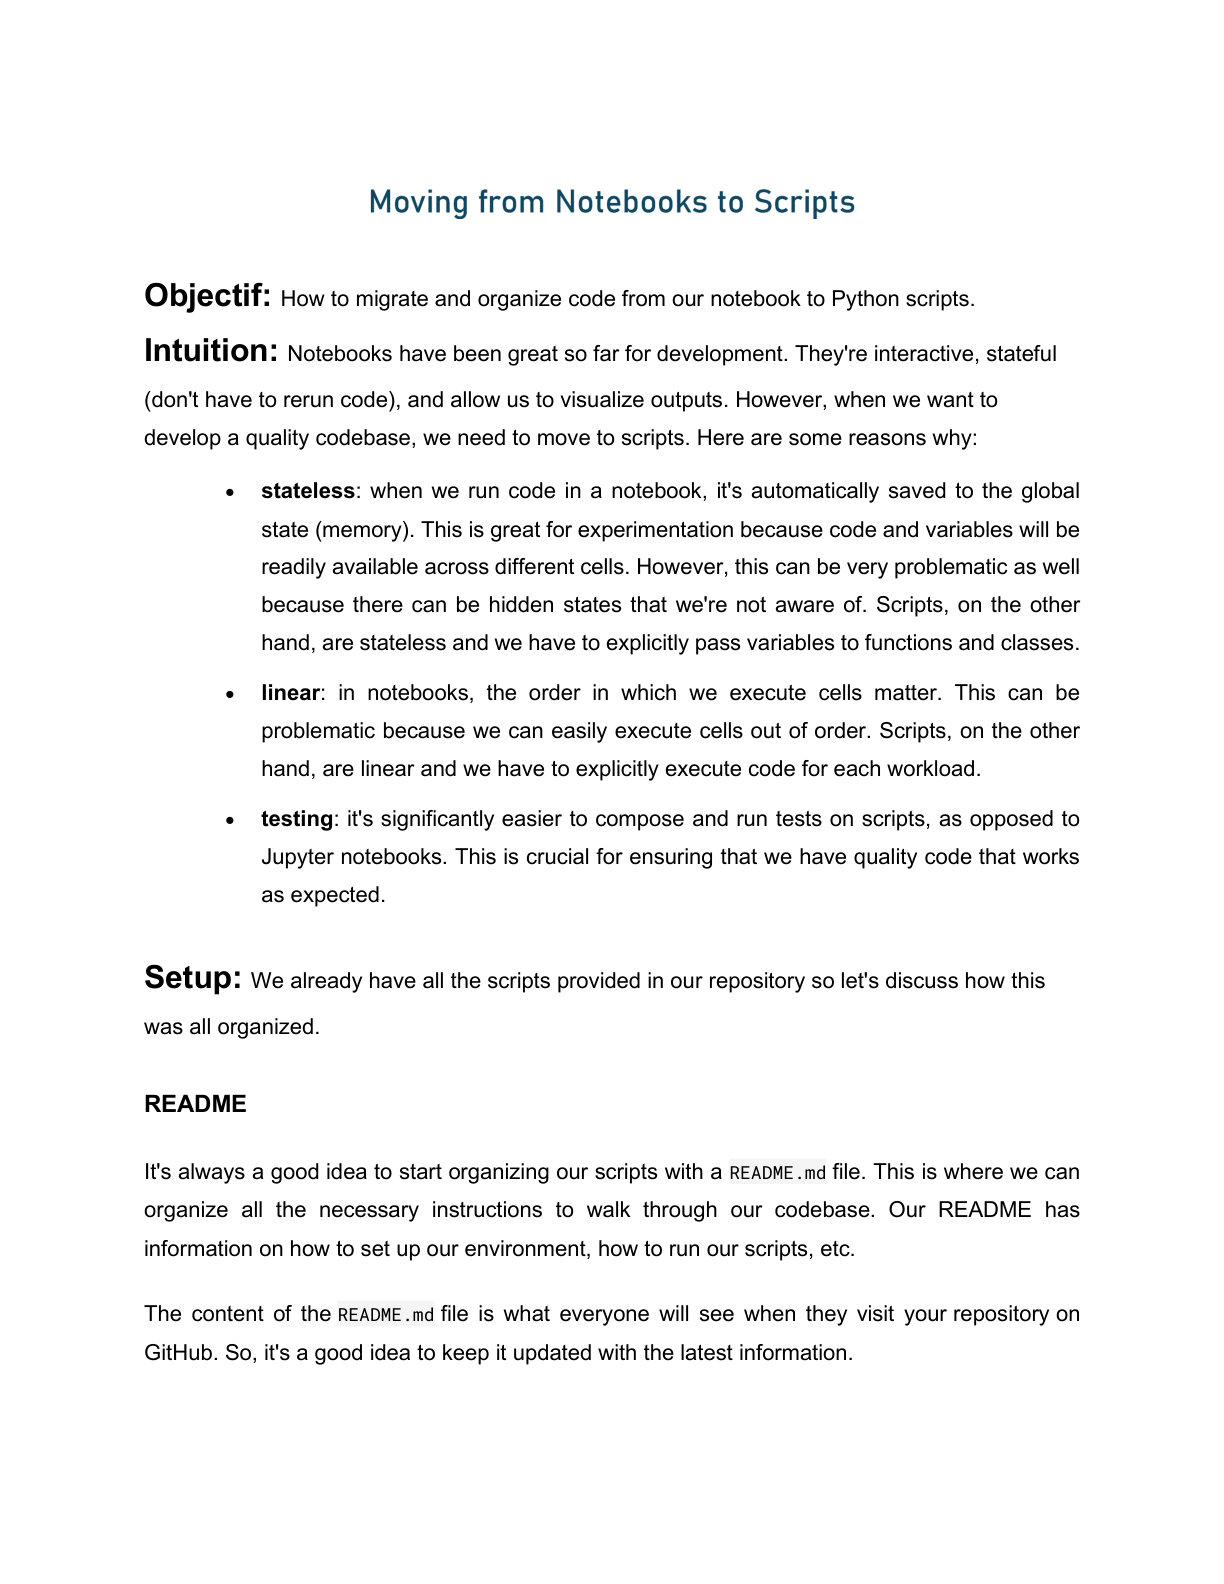
\includegraphics[width=0.72\textwidth]{figures/course_pdf_notebook_to_scripts.png}
    \caption{Course slide evidence: the first topic is moving from notebooks to scripts.}
    \label{fig:course-pdf}
\end{figure}

\subsection{Existing Notebook}

The original notebook is:

\begin{lstlisting}[style=projectcode]
MLOpsFull/mlops_Mine - Copy.ipynb
\end{lstlisting}

Its main sections include setup, data ingestion, preprocessing, training, experiment tracking, evaluation, interpretability, prediction, and serving. This is a typical research-to-development notebook: it contains the full workflow, but the logic is not yet presented as independent production components.

\subsection{Script-Based Architecture}

The notebook workflow has been separated into modules under \texttt{MLOpsFull/madewithml}. Each file owns a specific responsibility, which improves maintainability and makes the project easier to automate.

\begin{figure}[h]
    \centering
    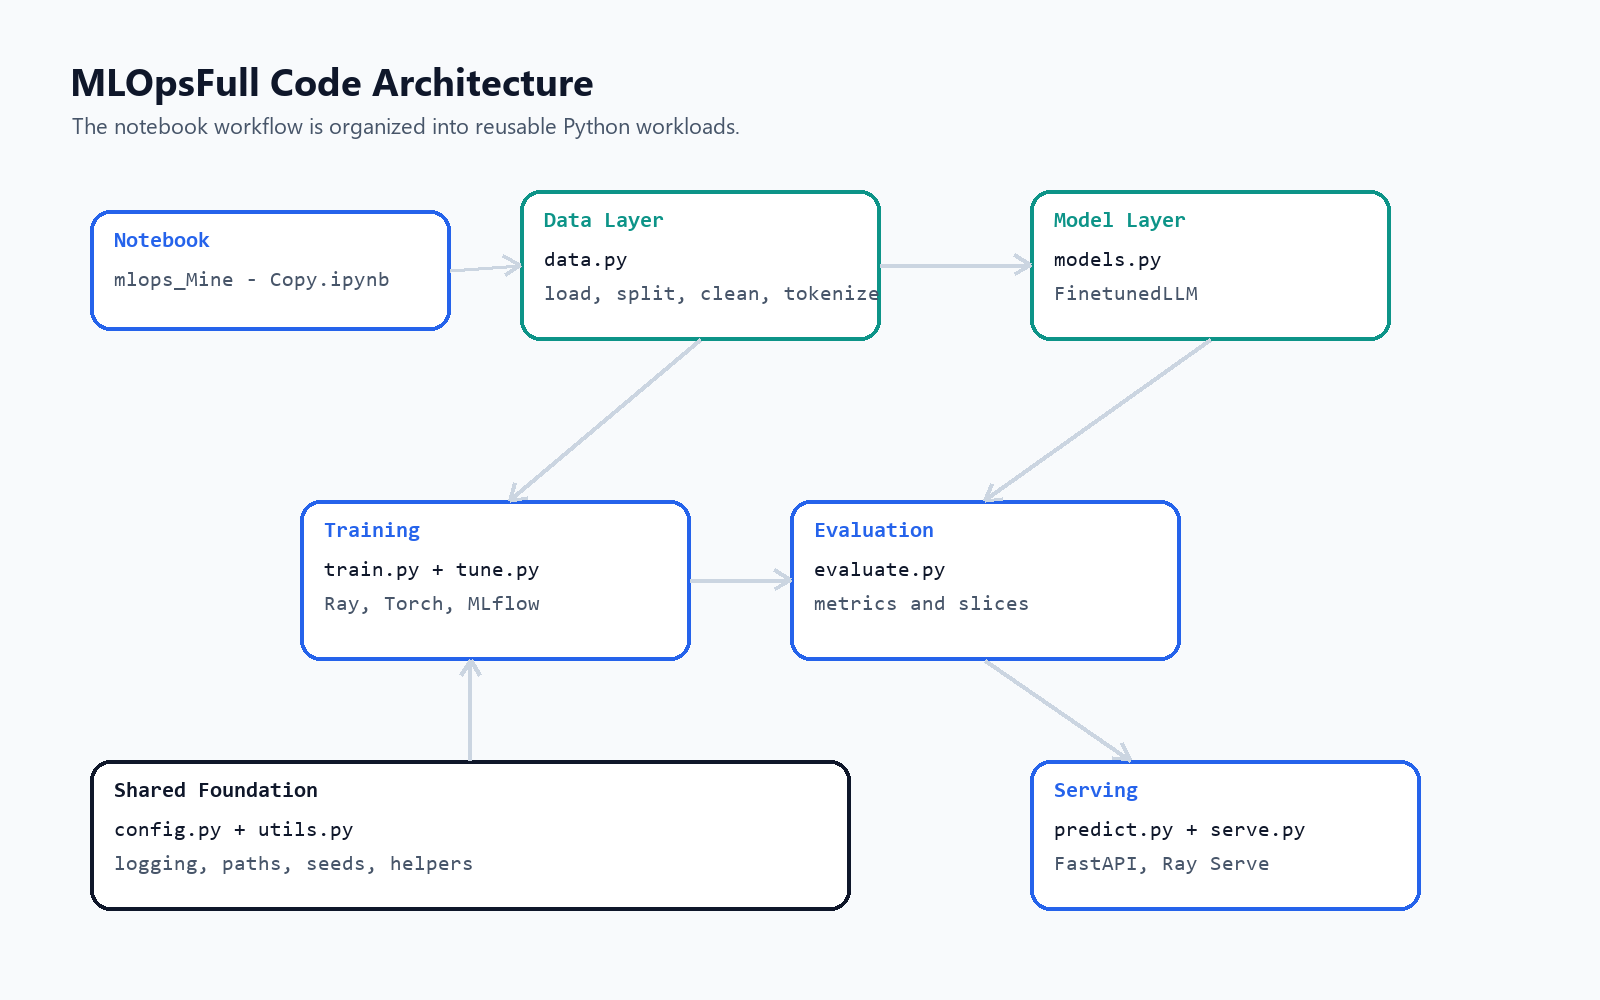
\includegraphics[width=0.96\textwidth]{figures/code_architecture.png}
    \caption{Script organization of the MLOpsFull project.}
    \label{fig:architecture}
\end{figure}

\subsection{Module Responsibilities}

\begin{longtable}{p{0.27\textwidth} p{0.63\textwidth}}
\toprule
\textbf{Module} & \textbf{Responsibility} \\
\midrule
\texttt{config.py} & Defines shared project configuration, logging paths, MLflow tracking URI, and constants such as stopwords. \\
\texttt{data.py} & Loads datasets, performs stratified splitting, cleans text, tokenizes input, and applies preprocessing. \\
\texttt{models.py} & Defines the PyTorch model architecture used for text classification. \\
\texttt{train.py} & Contains the Ray Train workload, training loop, checkpointing, and MLflow callback integration. \\
\texttt{tune.py} & Contains the hyperparameter tuning workload using Ray Tune and HyperOpt. \\
\texttt{evaluate.py} & Computes overall, per-class, and slice-level metrics. \\
\texttt{predict.py} & Loads model checkpoints and performs prediction or probability estimation. \\
\texttt{serve.py} & Defines the FastAPI application and Ray Serve deployment. \\
\texttt{utils.py} & Provides shared utility functions such as seed setting, batching, and dictionary saving. \\
\bottomrule
\end{longtable}

\subsection{Notebook-To-Script Mapping}

\begin{table}[h]
\centering
\begin{tabularx}{0.96\textwidth}{>{\bfseries}p{0.34\textwidth} X}
\toprule
Notebook Area & Script Destination \\
\midrule
Data loading and preprocessing & \texttt{madewithml/data.py} \\
Model definition & \texttt{madewithml/models.py} \\
Training loop & \texttt{madewithml/train.py} \\
Hyperparameter search & \texttt{madewithml/tune.py} \\
Evaluation & \texttt{madewithml/evaluate.py} \\
Prediction & \texttt{madewithml/predict.py} \\
Serving & \texttt{madewithml/serve.py} \\
Shared configuration & \texttt{madewithml/config.py} \\
Shared helpers & \texttt{madewithml/utils.py} \\
\bottomrule
\end{tabularx}
\caption{Mapping from notebook sections to production-oriented scripts.}
\end{table}

\subsection{Benefits For MLOps}

This structure is important because Jenkins, tests, model training jobs, and deployment commands all need scriptable entry points. A CI/CD server cannot reliably execute arbitrary notebook cells in a human-controlled order. It needs deterministic commands and modules.

The current organization creates a foundation for:

\begin{itemize}
    \item command-line training;
    \item automated evaluation;
    \item experiment tracking;
    \item API deployment;
    \item future Jenkins automation.
\end{itemize}

\section{Part 2: Logging For ML Systems}

\subsection{Purpose}

Logging records what happens inside the application during execution. In ML systems, logging is essential because failures can come from code, data, training configuration, model artifacts, infrastructure, or serving inputs.

Compared with \texttt{print}, logging is more suitable because it supports severity levels, multiple outputs, timestamps, persistent files, and consistent formatting.

\subsection{Logging Configuration In The Project}

The logging setup is defined in:

\begin{lstlisting}[style=projectcode]
MLOpsFull/madewithml/config.py
\end{lstlisting}

The project creates a \texttt{logs} directory and defines several handlers:

\begin{itemize}
    \item a console handler for terminal output;
    \item an \texttt{info.log} rotating file handler for informative logs;
    \item an \texttt{error.log} rotating file handler for errors.
\end{itemize}

Key implementation pattern:

\begin{lstlisting}[style=projectcode,language=Python]
LOGS_DIR = Path(ROOT_DIR, "logs")
LOGS_DIR.mkdir(parents=True, exist_ok=True)

logging_config = {
    "version": 1,
    "disable_existing_loggers": False,
    "handlers": {
        "console": {...},
        "info": {...},
        "error": {...},
    },
    "root": {
        "handlers": ["console", "info", "error"],
        "level": logging.INFO,
    },
}

logging.config.dictConfig(logging_config)
logger = logging.getLogger()
\end{lstlisting}

\subsection{Where Logs Are Used}

The project uses \texttt{logger.info(...)} to record important workflow outputs. For example:

\begin{itemize}
    \item training logs the timestamp, run ID, parameters, and metric history;
    \item evaluation logs overall metrics, per-class metrics, and slice metrics;
    \item prediction logs model prediction results.
\end{itemize}

\begin{figure}[h]
    \centering
    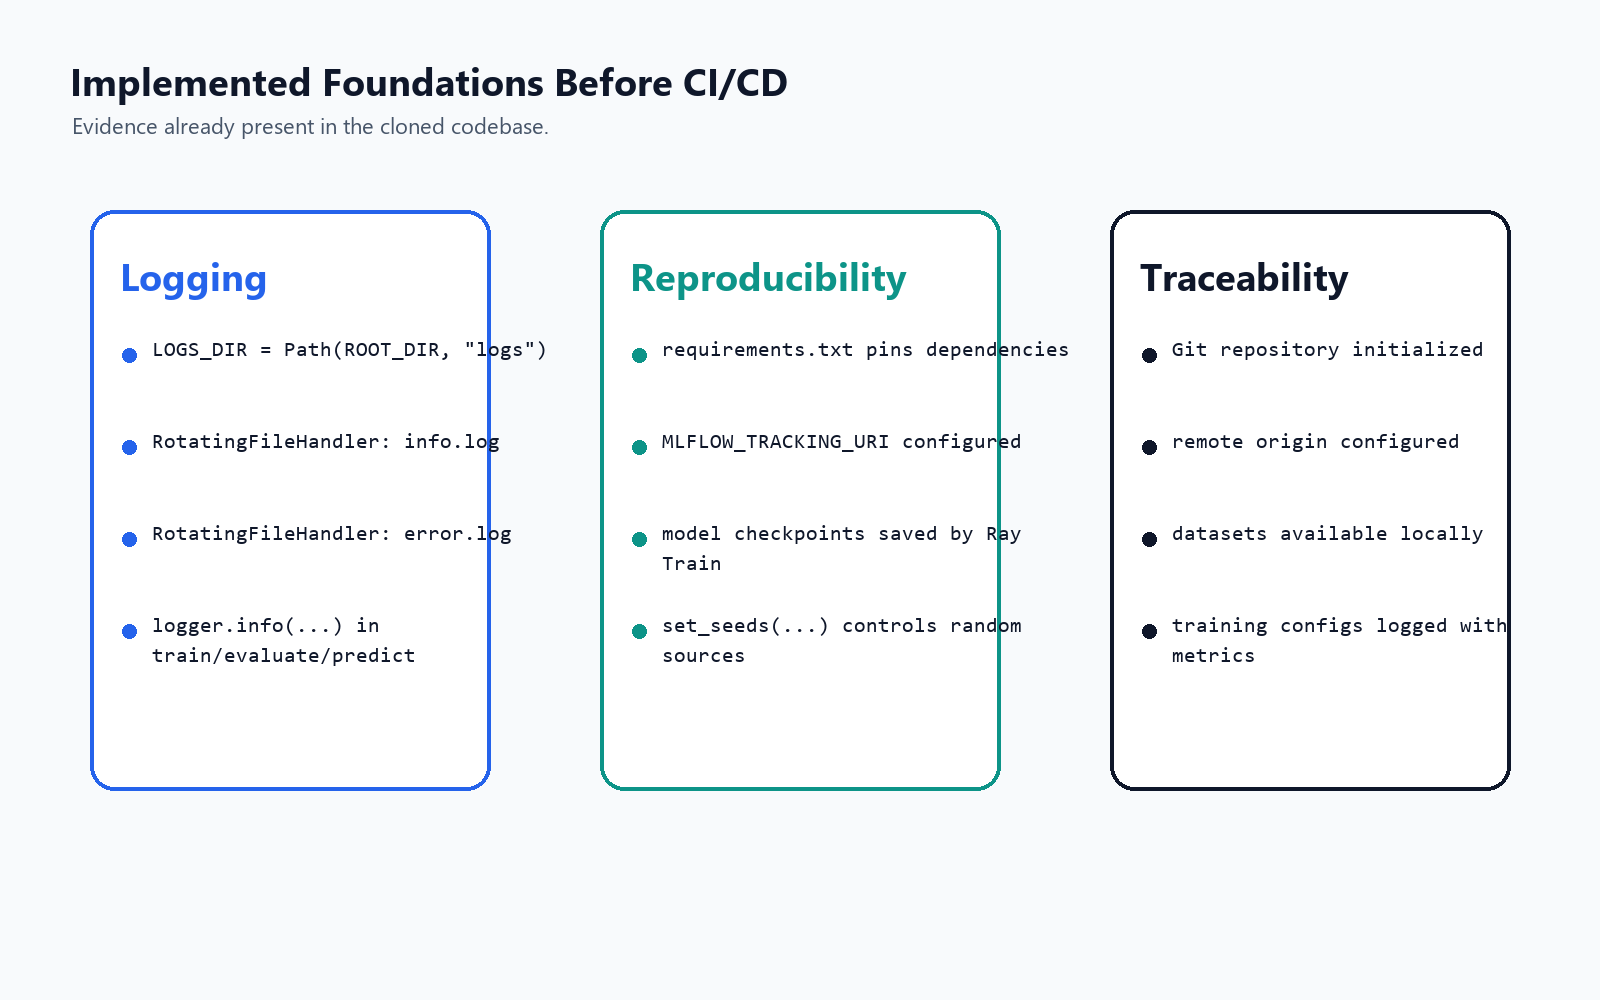
\includegraphics[width=0.96\textwidth]{figures/foundations_evidence.png}
    \caption{Evidence of implemented logging, reproducibility, and traceability foundations.}
    \label{fig:foundations}
\end{figure}

\subsection{Why Logging Matters For This Project}

In this project, logging supports three important MLOps needs:

\begin{enumerate}
    \item \textbf{Debugging}: errors and warnings can be inspected after a failed run.
    \item \textbf{Traceability}: training and evaluation outputs can be connected to model runs.
    \item \textbf{Monitoring readiness}: logs can later be exported to tools such as Loki, Elasticsearch, or cloud logging services and visualized in Grafana.
\end{enumerate}

\subsection{Production Extension}

For the final version, logs can be connected to the monitoring stack. A practical production-style design would be:

\begin{lstlisting}[style=projectcode]
Application logs -> Loki or Elasticsearch -> Grafana dashboards
\end{lstlisting}

This will allow the report to include screenshots of API errors, model prediction logs, and system events once the serving and monitoring stages are implemented.

\section{Part 3: Reproducibility}

\subsection{Purpose}

Reproducibility means being able to recreate a previous result. In machine learning, this is difficult because results depend on code, data, dependencies, random seeds, training parameters, model artifacts, and hardware.

A reproducible ML project should answer:

\begin{itemize}
    \item Which code version produced this model?
    \item Which dataset was used?
    \item Which dependencies were installed?
    \item Which parameters were used?
    \item Which metrics were obtained?
    \item Where is the model artifact stored?
\end{itemize}

\subsection{Code Versioning With Git}

The repositories are Git repositories and are connected to a remote origin. Git provides history, collaboration, rollback, and traceability.

\begin{lstlisting}[style=projectcode]
origin  https://github.com/AyoubMoutik/mlops-project.git
\end{lstlisting}

In the final report, screenshots from GitHub or Jenkins checkout logs can be added to strengthen this section.

\subsection{Dependency Versioning}

The project includes:

\begin{lstlisting}[style=projectcode]
MLOpsFull/requirements.txt
\end{lstlisting}

This file pins or constrains many important dependencies, including:

\begin{itemize}
    \item \texttt{mlflow}
    \item \texttt{ray}
    \item \texttt{torch}
    \item \texttt{transformers}
    \item \texttt{scikit-learn}
    \item \texttt{fastapi}
    \item \texttt{pytest}
    \item \texttt{great-expectations}
\end{itemize}

This is necessary because dependency changes can alter model behavior or break the pipeline.

\subsection{Data Versioning}

For this educational project, the datasets are stored directly in the repository:

\begin{lstlisting}[style=projectcode]
MLOpsFull/datasets/dataset.csv
MLOpsFull/datasets/holdout.csv
MLOpsFull/datasets/projects.csv
MLOpsFull/datasets/tags.csv
\end{lstlisting}

This is acceptable because the datasets are small. In production, larger datasets should not usually be stored directly in Git. Better options include:

\begin{itemize}
    \item DVC;
    \item Git LFS;
    \item S3 or another object store;
    \item Snowflake or another warehouse;
    \item versioned data lake storage.
\end{itemize}

\subsection{Model And Experiment Versioning With MLflow}

The project configures MLflow tracking in \texttt{config.py}. The model registry path is derived from the configured storage directory, and MLflow is set using a file URI.

\begin{lstlisting}[style=projectcode,language=Python]
MODEL_REGISTRY = Path(f"{EFS_DIR}/mlflow")
MLFLOW_TRACKING_URI = "file://" + str(MODEL_REGISTRY.absolute())
mlflow.set_tracking_uri(MLFLOW_TRACKING_URI)
\end{lstlisting}

During training, the project uses an MLflow callback:

\begin{lstlisting}[style=projectcode,language=Python]
mlflow_callback = MLflowLoggerCallback(
    tracking_uri=MLFLOW_TRACKING_URI,
    experiment_name=experiment_name,
    save_artifact=True,
)
\end{lstlisting}

This supports experiment tracking by storing parameters, metrics, checkpoints, and artifacts.

\subsection{Checkpointing}

The training workflow creates checkpoints and keeps the best checkpoint based on validation loss:

\begin{lstlisting}[style=projectcode,language=Python]
checkpoint_config = CheckpointConfig(
    num_to_keep=1,
    checkpoint_score_attribute="val_loss",
    checkpoint_score_order="min",
)
\end{lstlisting}

This matters because the best model can be loaded later for prediction, evaluation, or deployment.

\subsection{Random Seeds}

The project contains a utility function for setting random seeds. This reduces randomness across NumPy, Python, PyTorch, CUDA, and hashing behavior.

\begin{lstlisting}[style=projectcode,language=Python]
def set_seeds(seed: int = 42):
    np.random.seed(seed)
    random.seed(seed)
    torch.manual_seed(seed)
    torch.cuda.manual_seed(seed)
    os.environ["PYTHONHASHSEED"] = str(seed)
\end{lstlisting}

This does not guarantee perfect reproducibility on every machine, but it is an important baseline.

\subsection{Reproducibility Summary}

\begin{table}[h]
\centering
\begin{tabularx}{0.96\textwidth}{>{\bfseries}p{0.27\textwidth} X}
\toprule
Requirement & Current Project Evidence \\
\midrule
Code versioning & Git repository with remote origin configured. \\
Dependency versioning & \texttt{requirements.txt}. \\
Data availability & CSV datasets in \texttt{MLOpsFull/datasets}. \\
Experiment tracking & MLflow tracking URI and Ray MLflow callback. \\
Model artifact tracking & Ray checkpoints and MLflow artifacts. \\
Configuration tracking & Training parameters logged with results. \\
Randomness control & \texttt{set\_seeds} utility. \\
\bottomrule
\end{tabularx}
\caption{Current reproducibility mechanisms in the project.}
\end{table}

\section{Part 4: CI/CD With Jenkins}

\end{document}
